% Fig. 2 v3 -- generated by qualitatives_carla/pipeline/make_figure_tikz_v3.py. Do not edit by hand.
% Same preamble requirements and colour names as figures/architecture.tex.
\definecolor{ink}{HTML}{1F2A37}
\definecolor{egoedge}{HTML}{D48A2A}\definecolor{egotok}{HTML}{EFA54A}
\definecolor{denedge}{HTML}{4F82BE}\definecolor{lattok}{HTML}{6E9BD0}\definecolor{denfill}{HTML}{D4E4F4}
\definecolor{motfill}{HTML}{CFE6D3}\definecolor{recline}{HTML}{5B9F6D}
\definecolor{halo}{HTML}{0B0D10}
\begin{tikzpicture}[
  font=\sffamily\scriptsize,
  >={Stealth[length=4pt,width=3.5pt]},
  frame/.style={draw=ink!25,line width=0.4pt},
  panel/.style={font=\sffamily\footnotesize\bfseries,anchor=west,inner sep=0pt,text=ink},
  hdr/.style={font=\sffamily\scriptsize,anchor=south west,inner sep=0pt,text=ink},
  tag/.style={font=\sffamily\tiny,inner sep=0.55pt,rounded corners=0.5pt,fill=white,fill opacity=0.82,text opacity=1},
  tiny/.style={font=\sffamily\tiny,inner sep=0pt},
  small/.style={font=\sffamily\scriptsize,inner sep=0pt},
]

\node[panel] at (0.020,-0.280) {(a) Ego-vehicle camera};
\node[panel] at (7.756,-0.280) {(b) Generated motion over time};
\node[panel] at (15.491,-0.280) {(c) Samples $\mathbf{x}\sim p(\mathbf{x}\mid\mathbf{e})$};
% ---------------- row 0: Waymo M441_65 (sample 7 rendered) ----------------
\node[hdr] at (0.020,-0.910) {\textbf{Waymo, stopping example.} The recorded pedestrian and all eight generated samples stop.};
\node[inner sep=0pt,anchor=south west] at (0.020,-5.230) {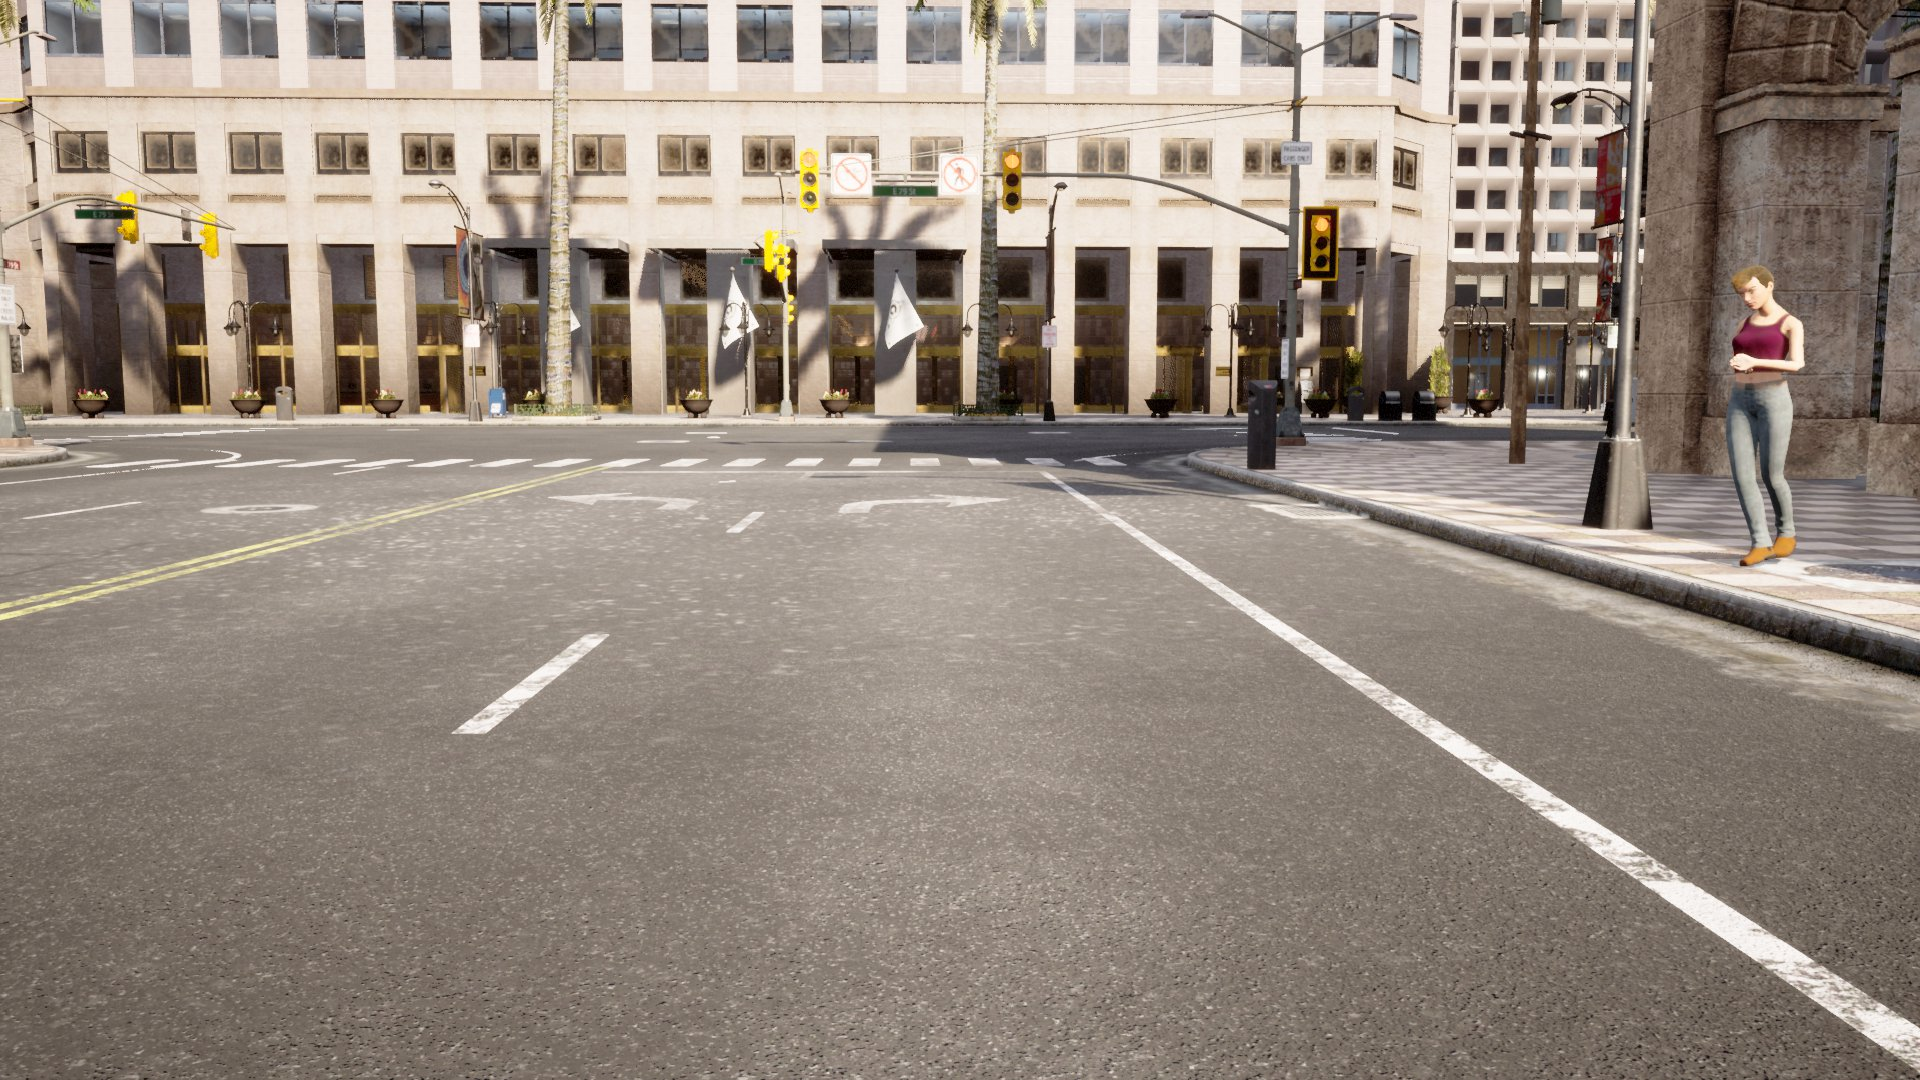
\includegraphics[width=7.556cm,height=4.250cm]{figures/carla_main_20261117/panels/16M_ego.jpg}};
\begin{scope}
  \clip (0.020,-5.230) rectangle (7.576,-0.980);
  \draw[halo,opacity=0.30,line width=2.55pt,line cap=round,line join=round] plot coordinates {(6.835,-3.225) (7.029,-3.242) (7.003,-3.235) (7.071,-3.229) (7.042,-3.258) (6.905,-3.278)};
  \draw[denedge,line width=1.35pt,line cap=round,line join=round] plot coordinates {(6.835,-3.225) (7.029,-3.242) (7.003,-3.235) (7.071,-3.229) (7.042,-3.258) (6.905,-3.278)};
  \node[tag,anchor=west,text=denedge] at (7.005,-3.258) {8.7\,s};
\end{scope}
\draw[frame] (0.020,-5.230) rectangle (7.576,-0.980);
\node[inner sep=0pt,anchor=south west] at (7.756,-5.230) {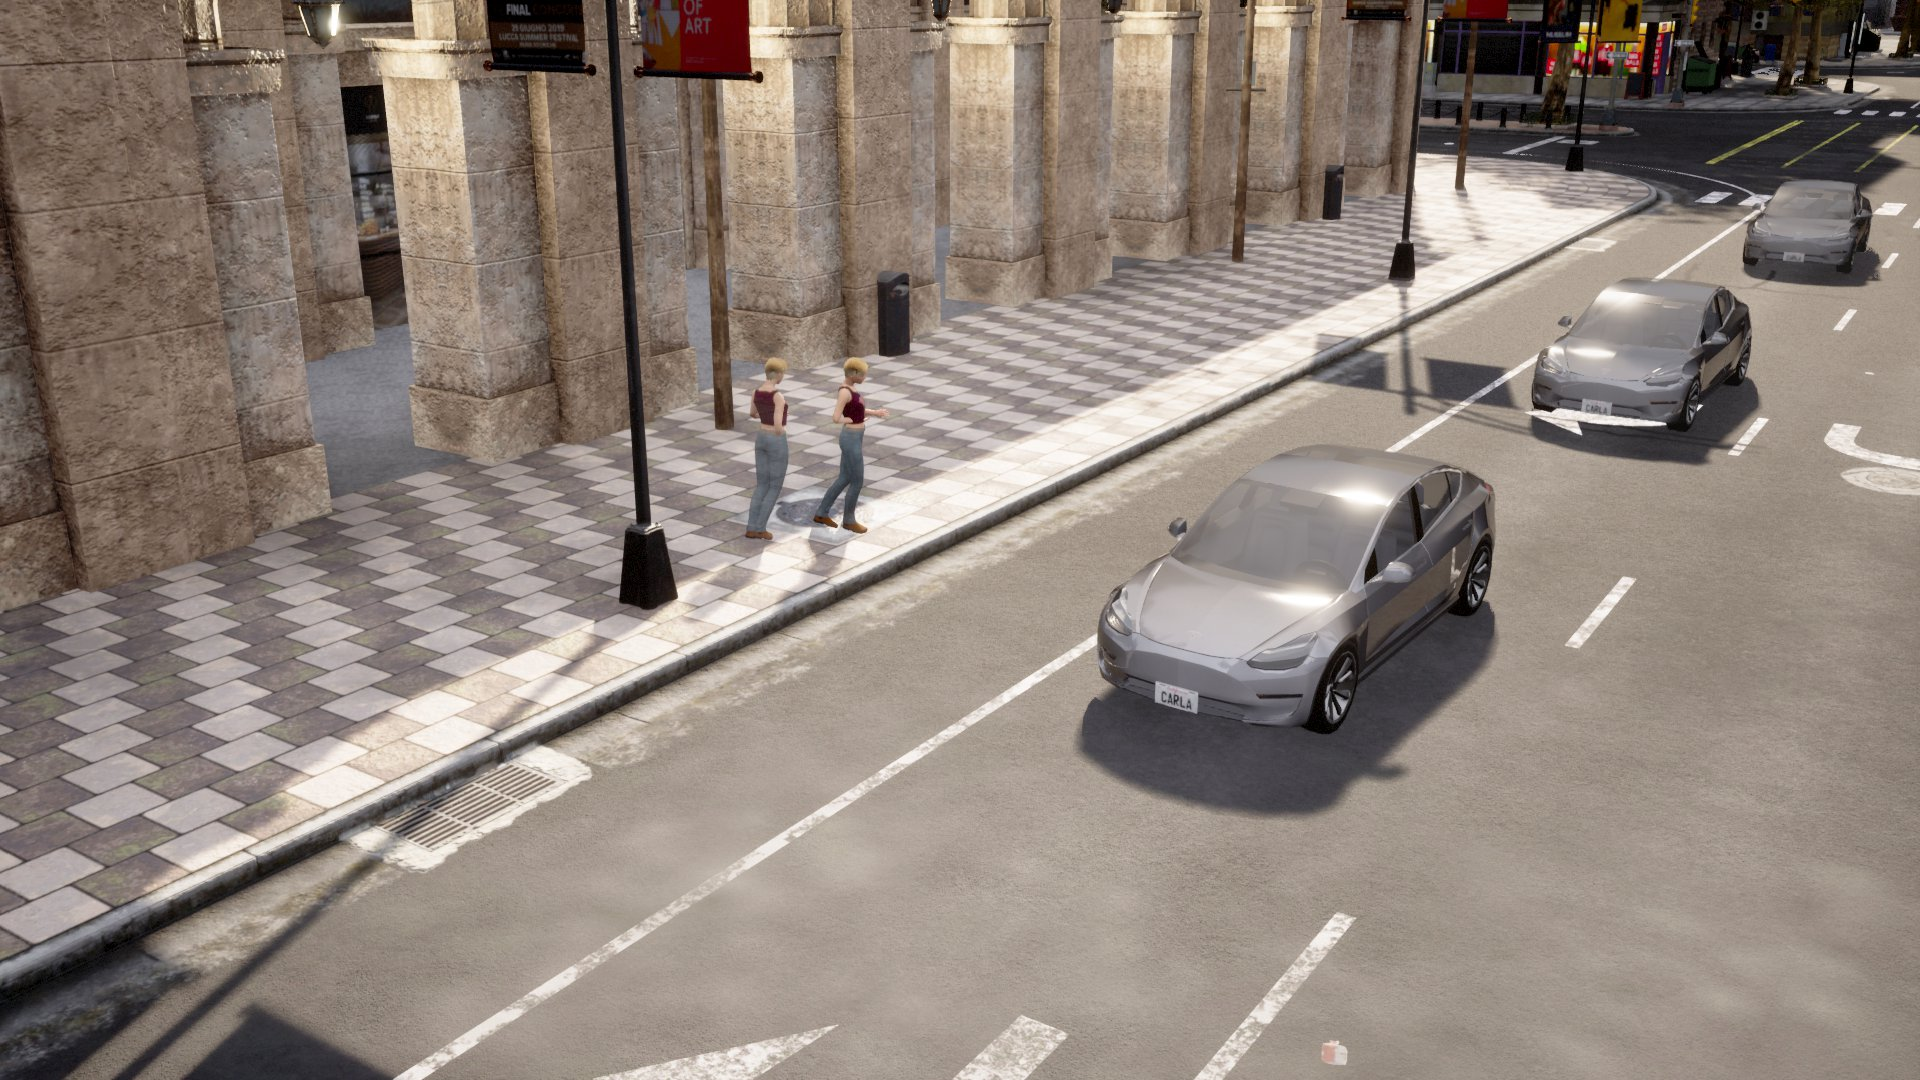
\includegraphics[width=7.556cm,height=4.250cm]{figures/carla_main_20261117/panels/16M_elevated.jpg}};
\begin{scope}
  \clip (7.756,-5.230) rectangle (15.311,-0.980);
  \draw[halo,opacity=0.30,line width=2.50pt,line cap=round,line join=round] plot coordinates {(15.147,-1.701) (14.729,-2.135) (14.581,-2.266)};
  \draw[egoedge,line width=1.30pt,line cap=round,line join=round] plot coordinates {(15.147,-1.701) (14.729,-2.135) (14.581,-2.266)};
  \draw[halo,opacity=0.30,line width=2.50pt,line cap=round] (14.581,-2.266) -- (12.914,-3.495);
  \draw[egoedge,line width=1.30pt,-{Stealth[length=5pt,width=4.5pt]}] (14.581,-2.266) -- (12.914,-3.495);
  \draw[halo,opacity=0.30,line width=2.30pt,line cap=round,line join=round] plot coordinates {(10.889,-3.168) (11.180,-3.149) (11.496,-3.213)};
  \draw[recline,line width=1.10pt,line cap=round,line join=round,opacity=0.92] plot coordinates {(10.889,-3.168) (11.180,-3.149) (11.496,-3.213)};
  \draw[halo,opacity=0.30,line width=2.55pt,line cap=round,line join=round] plot coordinates {(10.889,-3.168) (10.854,-3.137) (10.890,-3.129) (10.795,-3.135) (11.131,-3.117)};
  \draw[denedge,line width=1.35pt,line cap=round,line join=round] plot coordinates {(10.889,-3.168) (10.854,-3.137) (10.890,-3.129) (10.795,-3.135) (11.131,-3.117)};
  \node[tag,anchor=south,text=egoedge] at (14.919,-1.627) {3\,s};
  \node[tag,anchor=south,text=egoedge] at (14.292,-2.017) {6\,s};
  \node[tag,anchor=south,text=egoedge] at (12.968,-2.720) {8.7\,s};
  \node[tag,anchor=west,text=denedge] at (10.919,-3.116) {6\,s};
  \node[tag,anchor=west,text=denedge] at (11.231,-3.097) {8.7\,s};
\end{scope}
\draw[frame] (7.756,-5.230) rectangle (15.311,-0.980);
\begin{scope}
  \clip (15.491,-5.230) rectangle (20.380,-0.980);
  \draw[ink!12,line width=0.3pt] (15.647,-5.230) -- (15.647,-0.980);
  \draw[ink!12,line width=0.3pt] (16.580,-5.230) -- (16.580,-0.980);
  \draw[ink!12,line width=0.3pt] (17.513,-5.230) -- (17.513,-0.980);
  \draw[ink!12,line width=0.3pt] (18.446,-5.230) -- (18.446,-0.980);
  \draw[ink!12,line width=0.3pt] (19.379,-5.230) -- (19.379,-0.980);
  \draw[ink!12,line width=0.3pt] (20.313,-5.230) -- (20.313,-0.980);
  \draw[ink!12,line width=0.3pt] (15.491,-4.711) -- (20.380,-4.711);
  \draw[ink!12,line width=0.3pt] (15.491,-3.778) -- (20.380,-3.778);
  \draw[ink!12,line width=0.3pt] (15.491,-2.845) -- (20.380,-2.845);
  \draw[ink!12,line width=0.3pt] (15.491,-1.912) -- (20.380,-1.912);
  \draw[egoedge,line width=1.00pt,line cap=round,line join=round] plot coordinates {(29.156,11.652) (26.646,7.744) (24.531,4.386) (23.683,3.085) (22.405,1.239)};
  \draw[egoedge,line width=1.00pt,-{Stealth[length=4pt,width=3.5pt]}] (22.405,1.239) -- (18.754,-3.860);
  \draw[lattok,line width=0.55pt,line cap=round,line join=round,opacity=0.85] plot coordinates {(16.580,-2.845) (16.831,-2.729) (16.925,-2.657) (16.989,-2.585) (17.019,-2.519) (16.996,-2.488) (16.943,-2.475) (16.746,-2.472) (16.691,-2.450) (16.705,-2.413) (16.756,-2.374) (16.829,-2.354) (16.908,-2.351)};
  \draw[lattok,line width=0.55pt,line cap=round,line join=round,opacity=0.85] plot coordinates {(16.580,-2.845) (16.511,-2.714) (16.510,-2.635) (16.539,-2.583) (16.483,-2.586) (16.421,-2.566) (16.382,-2.602) (16.386,-2.625) (16.405,-2.639)};
  \draw[lattok,line width=0.55pt,line cap=round,line join=round,opacity=0.85] plot coordinates {(16.580,-2.845) (16.505,-2.747) (16.564,-2.752) (16.568,-2.737) (16.641,-2.750) (16.784,-2.718)};
  \draw[lattok,line width=0.55pt,line cap=round,line join=round,opacity=0.85] plot coordinates {(16.580,-2.845) (16.581,-2.908) (16.558,-2.907) (16.447,-2.793) (16.439,-2.756) (16.448,-2.717)};
  \draw[lattok,line width=0.55pt,line cap=round,line join=round,opacity=0.85] plot coordinates {(16.580,-2.845) (16.441,-2.845) (16.419,-2.822) (16.448,-2.791) (16.448,-2.819) (16.422,-2.823) (16.257,-2.767) (16.145,-2.803) (16.102,-2.886)};
  \draw[lattok,line width=0.55pt,line cap=round,line join=round,opacity=0.85] plot coordinates {(16.580,-2.845) (16.452,-2.816) (16.345,-2.660) (16.335,-2.715) (16.377,-2.679) (16.408,-2.629)};
  \draw[lattok,line width=0.55pt,line cap=round,line join=round,opacity=0.85] plot coordinates {(16.580,-2.845) (16.599,-2.810) (16.657,-2.792) (16.814,-2.798) (16.907,-2.828) (16.870,-2.743) (16.821,-2.732) (16.799,-2.756) (16.771,-2.837) (16.781,-2.909)};
  \draw[recline,line width=0.85pt,line cap=round,line join=round,opacity=0.95] plot coordinates {(16.580,-2.845) (16.797,-2.835) (16.920,-2.809) (16.918,-2.780) (17.031,-2.860) (17.240,-2.930) (17.293,-3.003)};
  \draw[denedge,line width=1.10pt,line cap=round,line join=round] plot coordinates {(16.580,-2.845) (16.528,-2.734) (16.533,-2.703) (16.568,-2.706) (16.541,-2.738) (16.480,-2.729) (16.453,-2.737) (16.457,-2.726) (16.555,-2.683) (16.654,-2.657) (16.854,-2.661)};
  \draw[white,fill=egoedge,line width=0.4pt] (18.754,-3.860) circle (0.95pt);
  \draw[white,fill=recline,line width=0.4pt] (17.293,-3.003) circle (0.95pt);
  \draw[white,fill=denedge,line width=0.4pt] (16.854,-2.661) circle (0.95pt);
  \node[tiny,anchor=south west,fill=white,fill opacity=0.82,text opacity=1,inner sep=0.4pt,text=egoedge] at (18.824,-3.820) {8.7};
  \draw[white,fill=recline,line width=0.4pt] (16.919,-2.809) circle (0.95pt);
  \draw[white,fill=denedge,line width=0.4pt] (16.487,-2.731) circle (0.95pt);
  \draw[white,fill=recline,line width=0.4pt] (16.902,-2.814) circle (0.95pt);
  \draw[white,fill=denedge,line width=0.4pt] (16.535,-2.702) circle (0.95pt);
  \draw[white,fill=recline,line width=0.4pt] (16.580,-2.845) circle (0.95pt);
  \draw[white,fill=denedge,line width=0.4pt] (16.580,-2.845) circle (0.95pt);
  \draw[ink,line width=0.7pt] (19.105,-4.933) -- (20.038,-4.933);
  \node[small,anchor=south,text=ink] at (19.571,-4.873) {2\,m};
\end{scope}
\node[small,anchor=north west,text=ink!70] at (15.611,-1.090) {8 generated samples};
\draw[frame] (15.491,-5.230) rectangle (20.380,-0.980);

% ---------------- row 1: nuScenes M005_1 (sample 2 rendered) ----------------
\node[hdr] at (0.020,-5.740) {\textbf{nuScenes, walking example.} The recorded pedestrian and all eight generated samples keep walking.};
\node[inner sep=0pt,anchor=south west] at (0.020,-10.060) {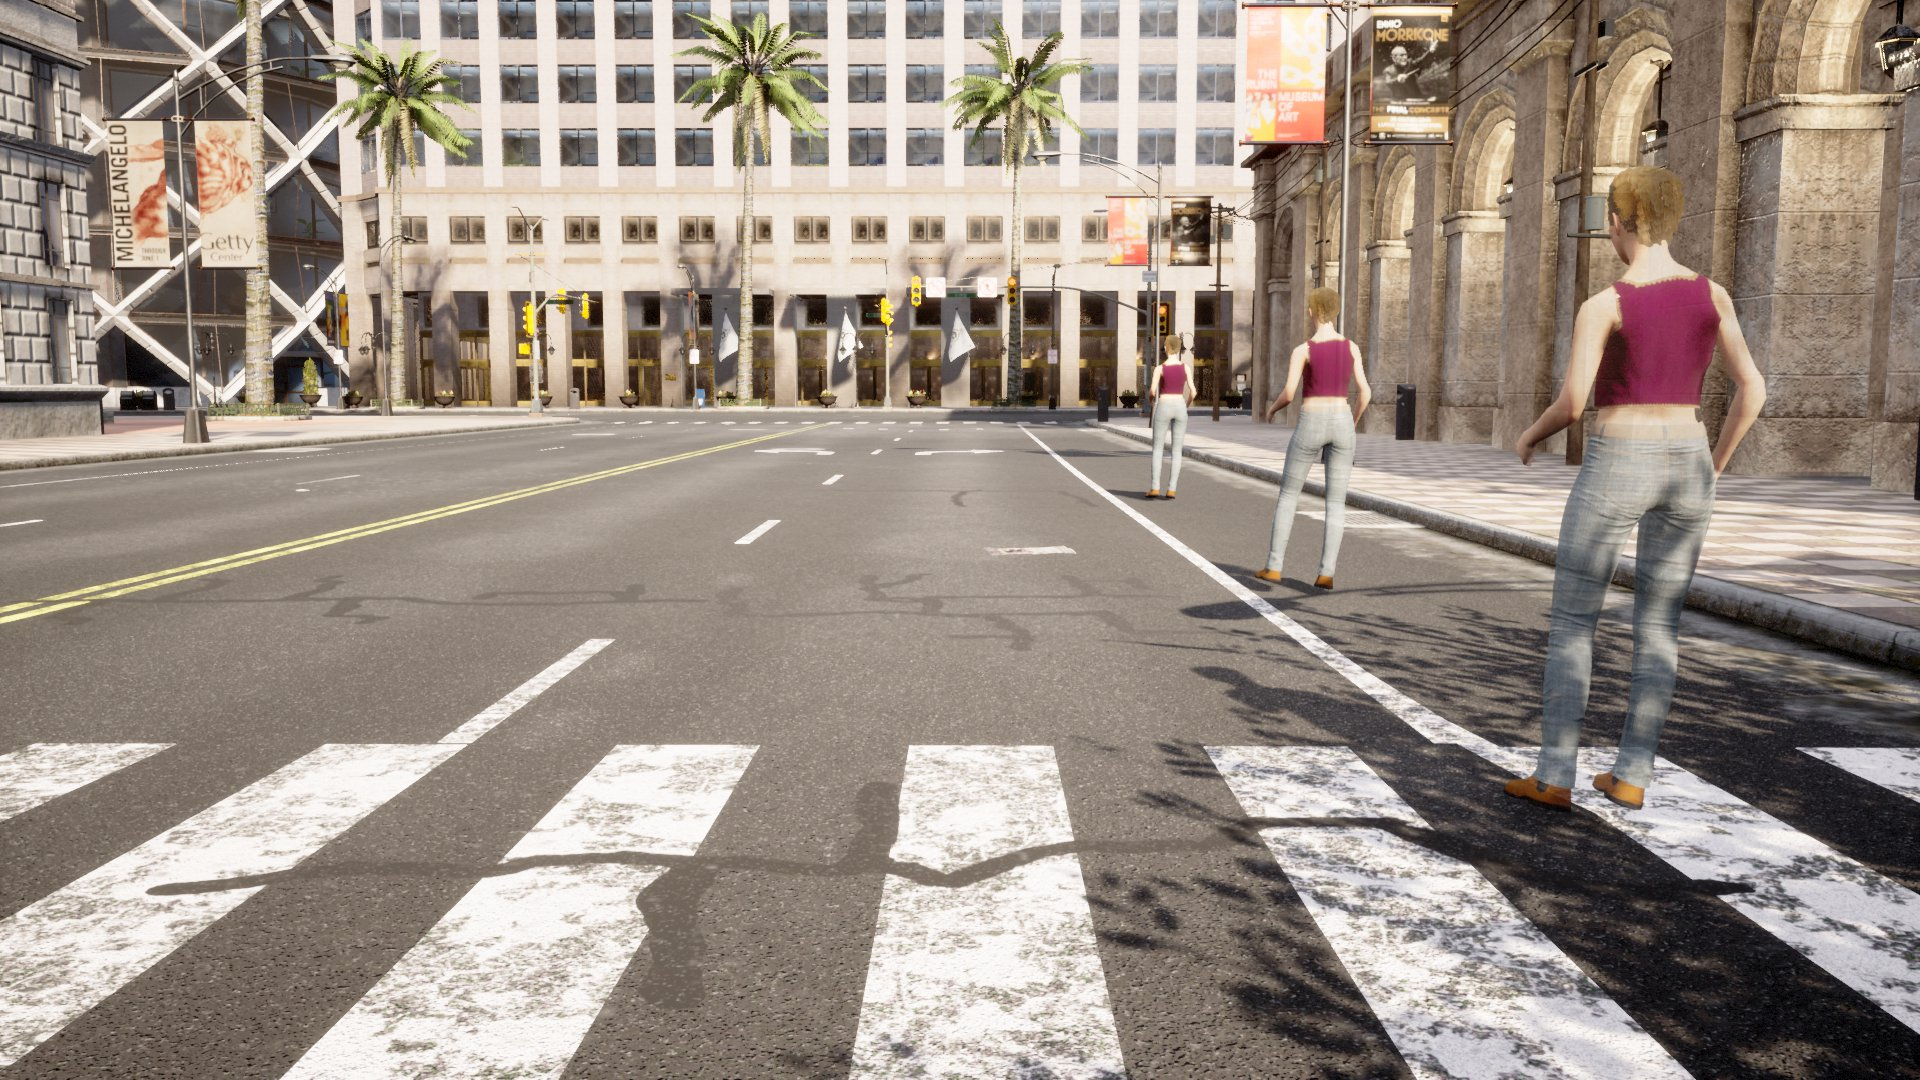
\includegraphics[width=7.556cm,height=4.250cm]{figures/carla_main_20261117/panels/08_ego.jpg}};
\begin{scope}
  \clip (0.020,-10.060) rectangle (7.576,-5.810);
  \draw[halo,opacity=0.30,line width=2.55pt,line cap=round,line join=round] plot coordinates {(6.399,-8.969) (5.594,-8.359)};
  \draw[denedge,line width=1.35pt,line cap=round,line join=round] plot coordinates {(6.399,-8.969) (5.594,-8.359)};
  \draw[halo,opacity=0.30,line width=2.55pt,line cap=round] (5.594,-8.359) -- (4.618,-7.762);
  \draw[denedge,line width=1.35pt,-{Stealth[length=5pt,width=4.5pt]}] (5.594,-8.359) -- (4.618,-7.762);
  \node[tag,anchor=west,text=denedge] at (6.499,-8.949) {0\,s};
  \node[tag,anchor=west,text=denedge] at (5.305,-8.093) {3\,s};
  \node[tag,anchor=west,text=denedge] at (4.718,-7.742) {7.6\,s};
\end{scope}
\draw[frame] (0.020,-10.060) rectangle (7.576,-5.810);
\node[inner sep=0pt,anchor=south west] at (7.756,-10.060) {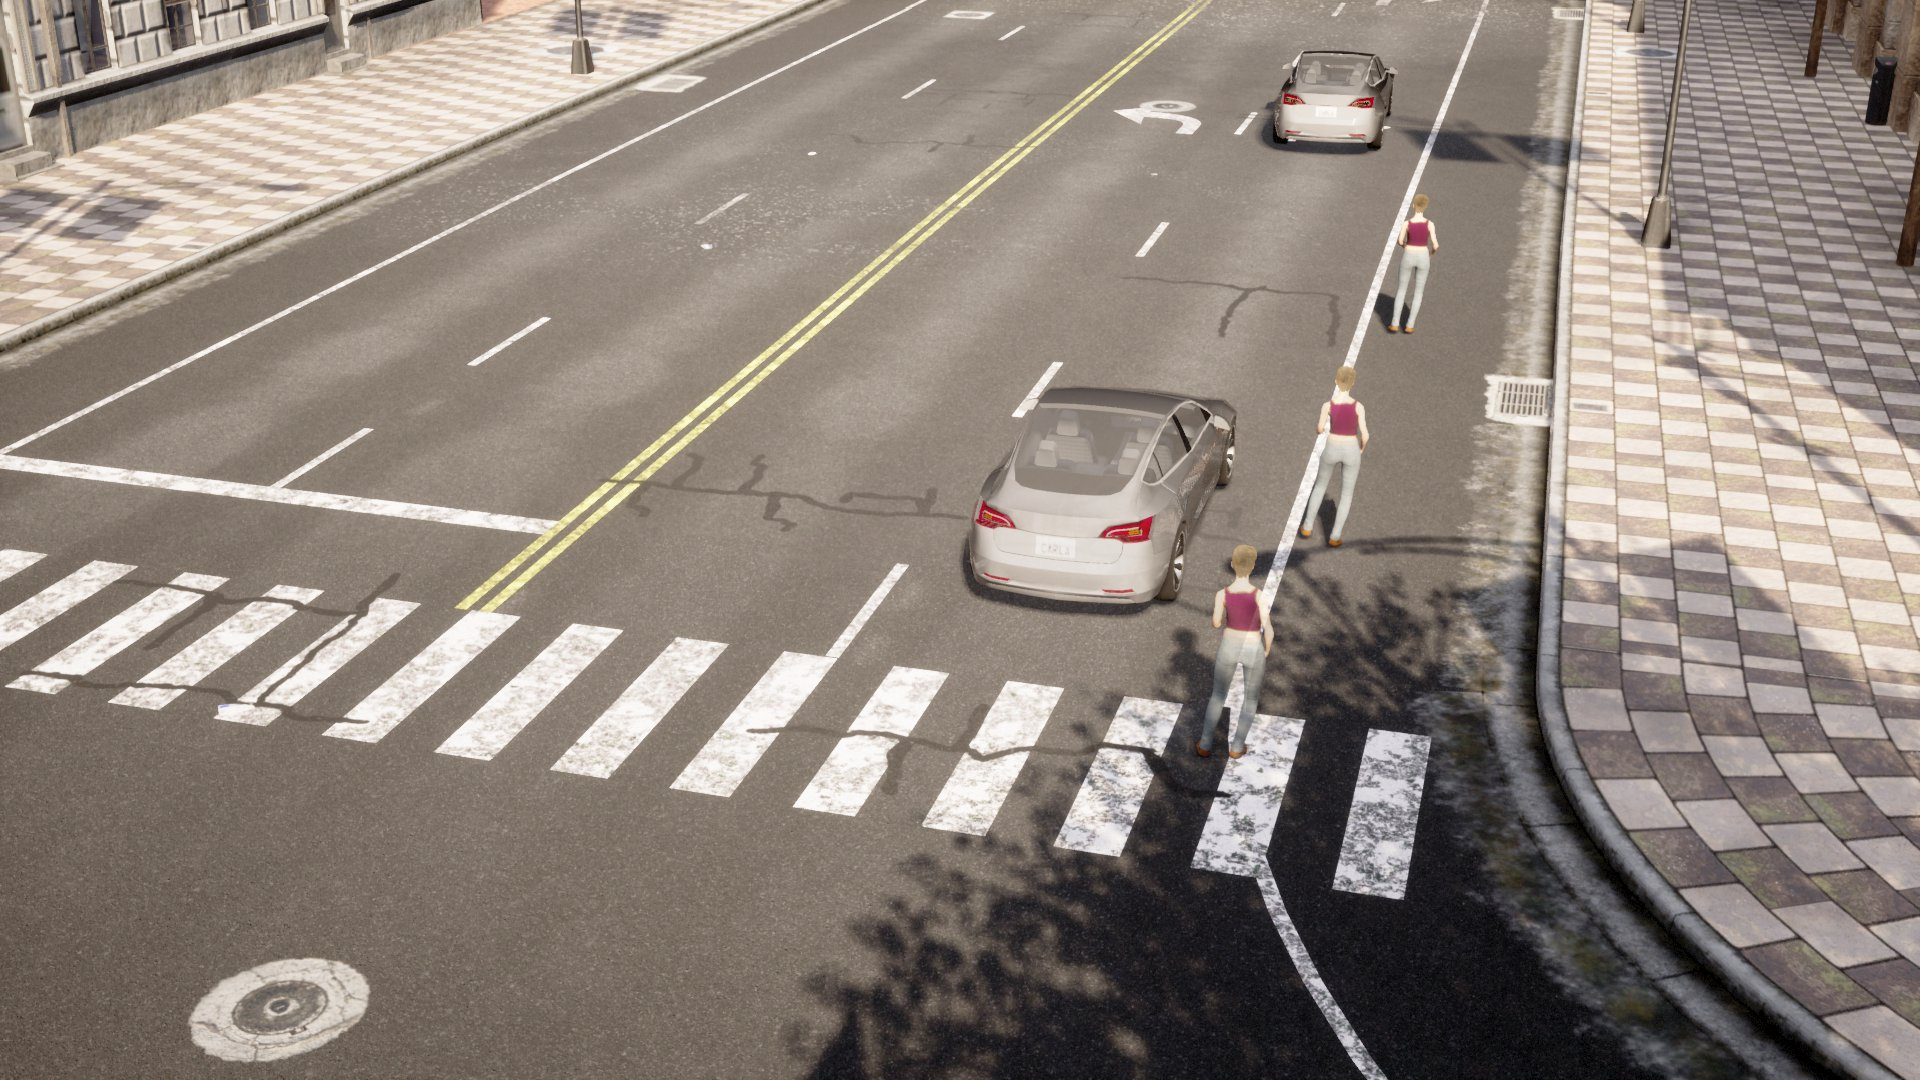
\includegraphics[width=7.556cm,height=4.250cm]{figures/carla_main_20261117/panels/08_elevated.jpg}};
\begin{scope}
  \clip (7.756,-10.060) rectangle (15.311,-5.810);
  \draw[halo,opacity=0.30,line width=2.50pt,line cap=round,line join=round] plot coordinates {(-14.301,-54.424) (8.879,-13.682) (10.520,-10.780) (11.982,-8.139)};
  \draw[egoedge,line width=1.30pt,line cap=round,line join=round] plot coordinates {(-14.301,-54.424) (8.879,-13.682) (10.520,-10.780) (11.982,-8.139)};
  \draw[halo,opacity=0.30,line width=2.50pt,line cap=round] (11.982,-8.139) -- (13.075,-6.046);
  \draw[egoedge,line width=1.30pt,-{Stealth[length=5pt,width=4.5pt]}] (11.982,-8.139) -- (13.075,-6.046);
  \draw[halo,opacity=0.30,line width=2.30pt,line cap=round,line join=round] plot coordinates {(12.612,-8.781) (13.003,-7.840) (13.166,-7.639) (13.311,-7.150)};
  \draw[recline,line width=1.10pt,line cap=round,line join=round,opacity=0.92] plot coordinates {(12.612,-8.781) (13.003,-7.840) (13.166,-7.639) (13.311,-7.150)};
  \draw[halo,opacity=0.30,line width=2.55pt,line cap=round,line join=round] plot coordinates {(12.612,-8.781) (12.862,-8.296) (12.970,-8.046)};
  \draw[denedge,line width=1.35pt,line cap=round,line join=round] plot coordinates {(12.612,-8.781) (12.862,-8.296) (12.970,-8.046)};
  \draw[halo,opacity=0.30,line width=2.55pt,line cap=round] (12.970,-8.046) -- (13.298,-7.106);
  \draw[denedge,line width=1.35pt,-{Stealth[length=5pt,width=4.5pt]}] (12.970,-8.046) -- (13.298,-7.106);
  \node[tag,anchor=south,text=egoedge] at (12.136,-7.233) {3\,s};
  \node[tag,anchor=south,text=egoedge] at (13.030,-6.030) {6\,s};
  \node[tag,anchor=west,text=denedge] at (12.712,-8.761) {0\,s};
  \node[tag,anchor=west,text=denedge] at (13.103,-7.916) {3\,s};
  \node[tag,anchor=west,text=denedge] at (13.398,-7.086) {7.6\,s};
\end{scope}
\draw[frame] (7.756,-10.060) rectangle (15.311,-5.810);
\begin{scope}
  \clip (15.491,-10.060) rectangle (20.380,-5.810);
  \draw[ink!12,line width=0.3pt] (15.904,-10.060) -- (15.904,-5.810);
  \draw[ink!12,line width=0.3pt] (17.814,-10.060) -- (17.814,-5.810);
  \draw[ink!12,line width=0.3pt] (19.724,-10.060) -- (19.724,-5.810);
  \draw[ink!12,line width=0.3pt] (15.491,-8.873) -- (20.380,-8.873);
  \draw[ink!12,line width=0.3pt] (15.491,-6.963) -- (20.380,-6.963);
  \draw[egoedge,line width=1.00pt,line cap=round,line join=round] plot coordinates {(16.277,-12.875) (16.922,-10.681) (17.622,-8.204)};
  \draw[egoedge,line width=1.00pt,-{Stealth[length=4pt,width=3.5pt]}] (17.622,-8.204) -- (18.303,-5.865);
  \draw[lattok,line width=0.55pt,line cap=round,line join=round,opacity=0.85] plot coordinates {(17.814,-8.873) (18.262,-7.536) (18.509,-6.691)};
  \draw[lattok,line width=0.55pt,line cap=round,line join=round,opacity=0.85] plot coordinates {(17.814,-8.873) (17.996,-8.301) (18.191,-7.744) (18.598,-6.761)};
  \draw[lattok,line width=0.55pt,line cap=round,line join=round,opacity=0.85] plot coordinates {(17.814,-8.873) (18.530,-6.670)};
  \draw[lattok,line width=0.55pt,line cap=round,line join=round,opacity=0.85] plot coordinates {(17.814,-8.873) (17.875,-8.634) (17.970,-8.358) (18.105,-8.030) (18.459,-7.293) (18.651,-6.756)};
  \draw[lattok,line width=0.55pt,line cap=round,line join=round,opacity=0.85] plot coordinates {(17.814,-8.873) (18.041,-8.210) (18.098,-7.999) (18.430,-7.134) (18.543,-6.735)};
  \draw[lattok,line width=0.55pt,line cap=round,line join=round,opacity=0.85] plot coordinates {(17.814,-8.873) (18.071,-8.056) (18.508,-6.899)};
  \draw[lattok,line width=0.55pt,line cap=round,line join=round,opacity=0.85] plot coordinates {(17.814,-8.873) (18.169,-7.674) (18.496,-6.679)};
  \draw[recline,line width=0.85pt,line cap=round,line join=round,opacity=0.95] plot coordinates {(17.814,-8.873) (18.124,-7.919) (18.256,-7.641) (18.504,-6.791)};
  \draw[denedge,line width=1.10pt,line cap=round,line join=round] plot coordinates {(17.814,-8.873) (18.066,-8.171)};
  \draw[denedge,line width=1.10pt,-{Stealth[length=4pt,width=3.5pt]}] (18.066,-8.171) -- (18.514,-6.698);
  \draw[white,fill=recline,line width=0.4pt] (18.504,-6.791) circle (0.95pt);
  \draw[white,fill=denedge,line width=0.4pt] (18.514,-6.698) circle (0.95pt);
  \draw[white,fill=recline,line width=0.4pt] (18.369,-7.236) circle (0.95pt);
  \draw[white,fill=denedge,line width=0.4pt] (18.383,-7.175) circle (0.95pt);
  \draw[white,fill=egoedge,line width=0.4pt] (17.681,-7.997) circle (0.95pt);
  \draw[white,fill=recline,line width=0.4pt] (18.078,-8.061) circle (0.95pt);
  \draw[white,fill=denedge,line width=0.4pt] (18.104,-8.041) circle (0.95pt);
  \node[tiny,anchor=south west,fill=white,fill opacity=0.82,text opacity=1,inner sep=0.4pt,text=egoedge] at (17.751,-7.957) {3};
  \draw[white,fill=recline,line width=0.4pt] (17.814,-8.873) circle (0.95pt);
  \draw[white,fill=denedge,line width=0.4pt] (17.814,-8.873) circle (0.95pt);
  \draw[ink,line width=0.7pt] (18.128,-9.763) -- (20.038,-9.763);
  \node[small,anchor=south,text=ink] at (19.083,-9.703) {10\,m};
\end{scope}
\node[small,anchor=north west,text=ink!70] at (15.611,-5.920) {8 generated samples};
\draw[frame] (15.491,-10.060) rectangle (20.380,-5.810);

% ---------------- row 2: Staged 0008_37 (sample 7 rendered) ----------------
\node[hdr] at (0.020,-10.570) {\textbf{Staged, failure case.} The recorded pedestrian crosses. All eight generated samples stop before completing the crossing.};
\node[inner sep=0pt,anchor=south west] at (0.020,-14.890) {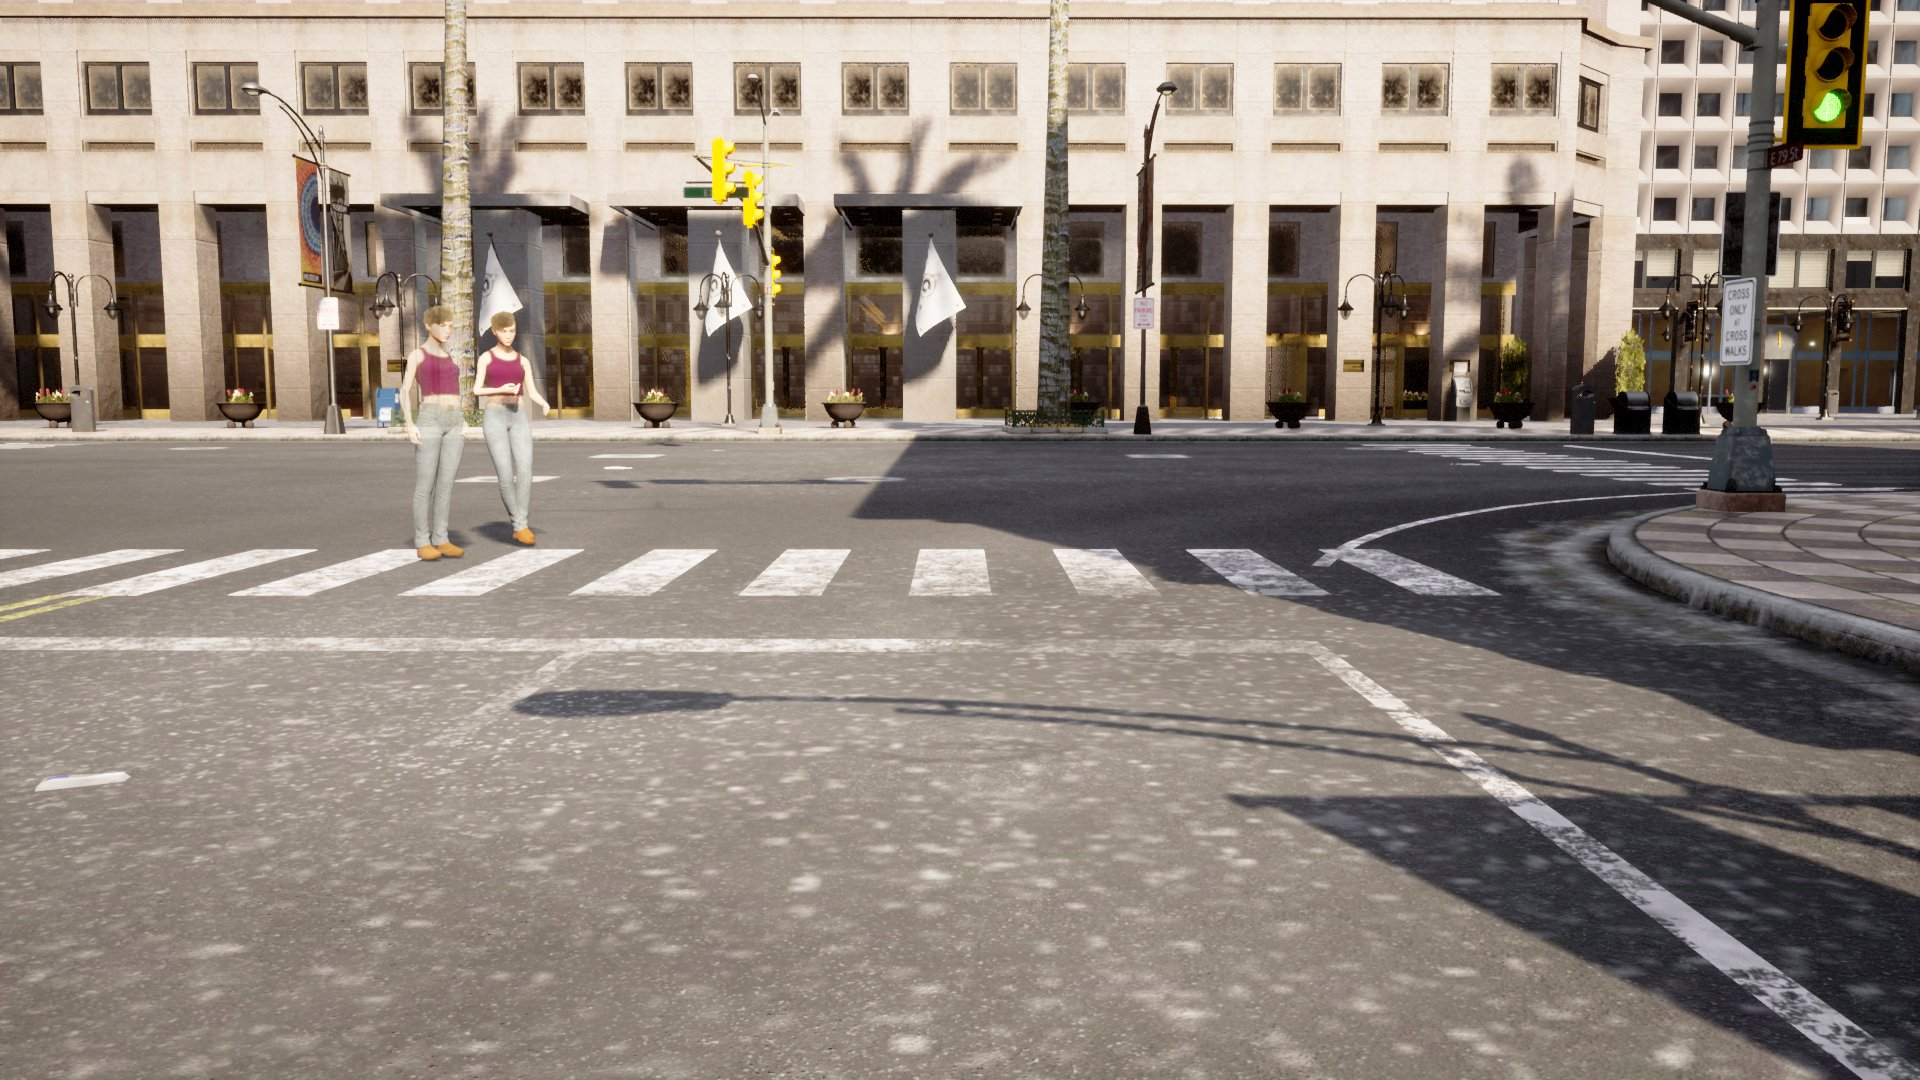
\includegraphics[width=7.556cm,height=4.250cm]{figures/carla_main_20261117/panels/02M_ego.jpg}};
\begin{scope}
  \clip (0.020,-14.890) rectangle (7.576,-10.640);
  \draw[halo,opacity=0.30,line width=2.55pt,line cap=round,line join=round] plot coordinates {(1.803,-12.825) (1.778,-12.811) (1.857,-12.788) (2.035,-12.770)};
  \draw[denedge,line width=1.35pt,line cap=round,line join=round] plot coordinates {(1.803,-12.825) (1.778,-12.811) (1.857,-12.788) (2.035,-12.770)};
  \node[tag,anchor=west,text=denedge] at (1.887,-12.800) {3\,s};
  \node[tag,anchor=west,text=denedge] at (2.135,-12.750) {8.5\,s};
\end{scope}
\draw[frame] (0.020,-14.890) rectangle (7.576,-10.640);
\node[inner sep=0pt,anchor=south west] at (7.756,-14.890) {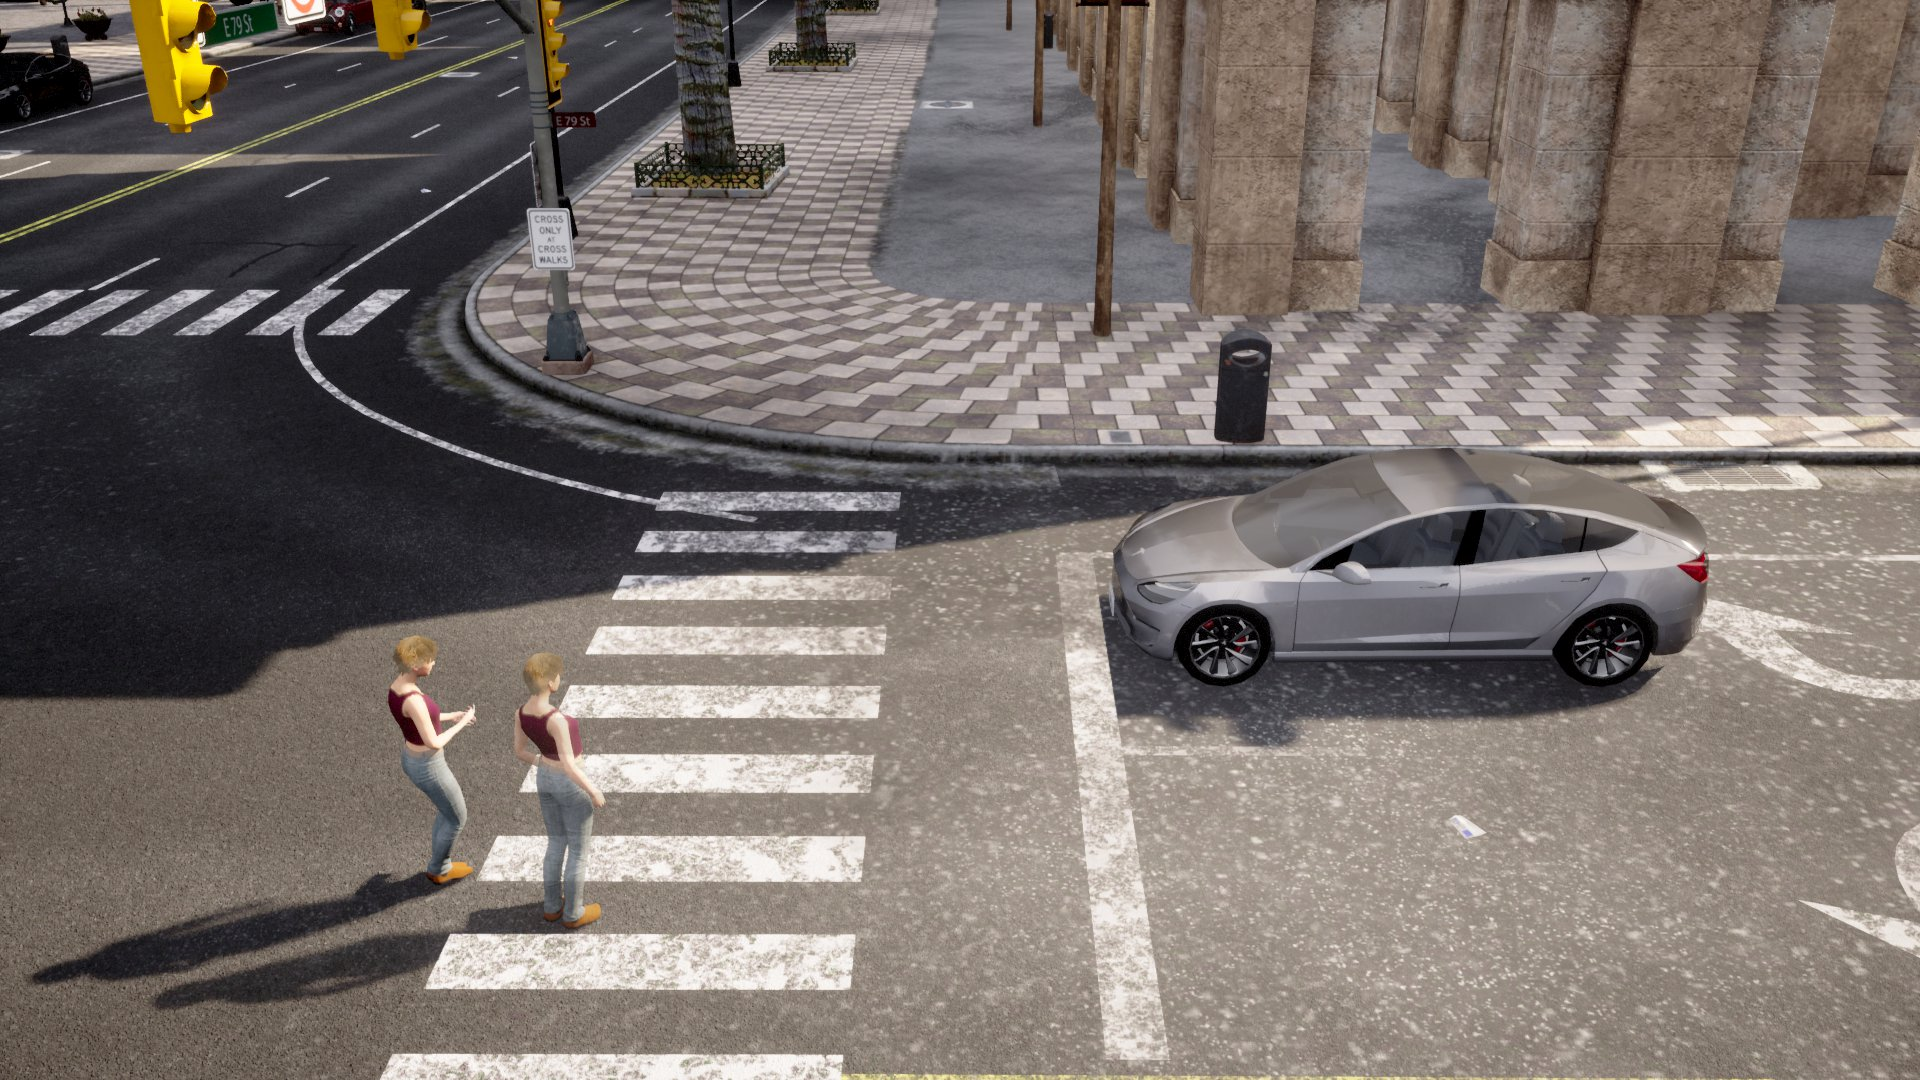
\includegraphics[width=7.556cm,height=4.250cm]{figures/carla_main_20261117/panels/02M_elevated.jpg}};
\begin{scope}
  \clip (7.756,-14.890) rectangle (15.311,-10.640);
  \draw[halo,opacity=0.30,line width=2.50pt,line cap=round] (21.905,-13.151) -- (13.241,-13.130);
  \draw[egoedge,line width=1.30pt,-{Stealth[length=5pt,width=4.5pt]}] (21.905,-13.151) -- (13.241,-13.130);
  \draw[halo,opacity=0.30,line width=2.30pt,line cap=round,line join=round] plot coordinates {(10.089,-14.176) (10.181,-14.101) (10.204,-13.958) (10.241,-13.872) (10.382,-13.801) (10.418,-13.748) (10.395,-13.683) (10.304,-13.581) (10.361,-13.443) (10.355,-13.291) (10.380,-13.215) (10.317,-13.127) (10.328,-13.079) (10.446,-12.837) (10.662,-12.542) (10.687,-12.476) (10.754,-12.414)};
  \draw[recline,line width=1.10pt,line cap=round,line join=round,opacity=0.92] plot coordinates {(10.089,-14.176) (10.181,-14.101) (10.204,-13.958) (10.241,-13.872) (10.382,-13.801) (10.418,-13.748) (10.395,-13.683) (10.304,-13.581) (10.361,-13.443) (10.355,-13.291) (10.380,-13.215) (10.317,-13.127) (10.328,-13.079) (10.446,-12.837) (10.662,-12.542) (10.687,-12.476) (10.754,-12.414)};
  \draw[halo,opacity=0.30,line width=2.55pt,line cap=round,line join=round] plot coordinates {(10.089,-14.176) (9.921,-14.226) (9.647,-14.217) (9.531,-14.174) (9.514,-14.156) (9.527,-14.123) (9.514,-14.127)};
  \draw[denedge,line width=1.35pt,line cap=round,line join=round] plot coordinates {(10.089,-14.176) (9.921,-14.226) (9.647,-14.217) (9.531,-14.174) (9.514,-14.156) (9.527,-14.123) (9.514,-14.127)};
  \node[tag,anchor=south,text=egoedge] at (13.338,-12.363) {8.5\,s};
  \node[tag,anchor=west,text=denedge] at (10.134,-14.178) {3\,s};
  \node[tag,anchor=west,text=denedge] at (9.614,-14.107) {8.5\,s};
\end{scope}
\draw[frame] (7.756,-14.890) rectangle (15.311,-10.640);
\begin{scope}
  \clip (15.491,-14.890) rectangle (20.380,-10.640);
  \draw[ink!12,line width=0.3pt] (16.397,-14.890) -- (16.397,-10.640);
  \draw[ink!12,line width=0.3pt] (17.655,-14.890) -- (17.655,-10.640);
  \draw[ink!12,line width=0.3pt] (18.913,-14.890) -- (18.913,-10.640);
  \draw[ink!12,line width=0.3pt] (20.170,-14.890) -- (20.170,-10.640);
  \draw[ink!12,line width=0.3pt] (15.491,-14.815) -- (20.380,-14.815);
  \draw[ink!12,line width=0.3pt] (15.491,-13.557) -- (20.380,-13.557);
  \draw[ink!12,line width=0.3pt] (15.491,-12.299) -- (20.380,-12.299);
  \draw[ink!12,line width=0.3pt] (15.491,-11.042) -- (20.380,-11.042);
  \draw[egoedge,line width=1.00pt,-{Stealth[length=4pt,width=3.5pt]}] (22.598,-12.667) -- (17.912,-12.643);
  \draw[lattok,line width=0.55pt,line cap=round,line join=round,opacity=0.85] plot coordinates {(16.397,-13.557) (16.343,-13.612) (16.291,-13.633) (16.215,-13.610) (16.183,-13.587) (16.145,-13.588) (16.132,-13.560) (16.158,-13.504) (16.126,-13.547) (16.151,-13.571)};
  \draw[lattok,line width=0.55pt,line cap=round,line join=round,opacity=0.85] plot coordinates {(16.397,-13.557) (16.296,-13.680) (16.277,-13.686) (16.275,-13.648) (16.270,-13.747) (16.288,-13.842)};
  \draw[lattok,line width=0.55pt,line cap=round,line join=round,opacity=0.85] plot coordinates {(16.397,-13.557) (16.435,-13.613) (16.304,-13.662) (16.259,-13.645) (16.254,-13.666) (16.278,-13.722)};
  \draw[lattok,line width=0.55pt,line cap=round,line join=round,opacity=0.85] plot coordinates {(16.397,-13.557) (16.386,-13.546) (16.203,-13.564) (16.178,-13.533) (16.194,-13.515)};
  \draw[lattok,line width=0.55pt,line cap=round,line join=round,opacity=0.85] plot coordinates {(16.397,-13.557) (16.322,-13.810) (16.265,-13.904) (16.211,-13.899) (16.029,-13.995)};
  \draw[lattok,line width=0.55pt,line cap=round,line join=round,opacity=0.85] plot coordinates {(16.397,-13.557) (16.387,-13.550) (16.178,-13.611) (16.136,-13.572) (16.139,-13.503) (16.122,-13.504) (16.133,-13.532)};
  \draw[lattok,line width=0.55pt,line cap=round,line join=round,opacity=0.85] plot coordinates {(16.397,-13.557) (16.345,-13.606) (16.038,-13.659) (15.992,-13.697)};
  \draw[recline,line width=0.85pt,line cap=round,line join=round,opacity=0.95] plot coordinates {(16.397,-13.557) (16.424,-13.507) (16.416,-13.344) (16.468,-13.289) (16.477,-13.246) (16.457,-13.193) (16.399,-13.105) (16.402,-12.977) (16.372,-12.823) (16.370,-12.741) (16.318,-12.640) (16.313,-12.582) (16.325,-12.261) (16.391,-11.782) (16.392,-11.658) (16.423,-11.536)};
  \draw[denedge,line width=1.10pt,line cap=round,line join=round] plot coordinates {(16.397,-13.557) (16.337,-13.589) (16.226,-13.583) (16.171,-13.556) (16.155,-13.525)};
  \draw[white,fill=egoedge,line width=0.4pt] (17.912,-12.643) circle (0.95pt);
  \draw[white,fill=recline,line width=0.4pt] (16.423,-11.536) circle (0.95pt);
  \draw[white,fill=denedge,line width=0.4pt] (16.155,-13.525) circle (0.95pt);
  \node[tiny,anchor=south west,fill=white,fill opacity=0.82,text opacity=1,inner sep=0.4pt,text=egoedge] at (17.982,-12.603) {8.5};
  \draw[white,fill=egoedge,line width=0.4pt] (18.246,-12.639) circle (0.95pt);
  \draw[white,fill=recline,line width=0.4pt] (16.322,-12.345) circle (0.95pt);
  \draw[white,fill=denedge,line width=0.4pt] (16.214,-13.579) circle (0.95pt);
  \draw[white,fill=egoedge,line width=0.4pt] (19.352,-12.651) circle (0.95pt);
  \draw[white,fill=recline,line width=0.4pt] (16.399,-13.105) circle (0.95pt);
  \draw[white,fill=denedge,line width=0.4pt] (16.378,-13.571) circle (0.95pt);
  \node[tiny,anchor=south west,fill=white,fill opacity=0.82,text opacity=1,inner sep=0.4pt,text=egoedge] at (19.422,-12.611) {3};
  \draw[white,fill=recline,line width=0.4pt] (16.397,-13.557) circle (0.95pt);
  \draw[white,fill=denedge,line width=0.4pt] (16.397,-13.557) circle (0.95pt);
  \draw[ink,line width=0.7pt] (18.780,-14.593) -- (20.038,-14.593);
  \node[small,anchor=south,text=ink] at (19.409,-14.533) {5\,m};
\end{scope}
\node[small,anchor=north west,text=ink!70] at (15.611,-10.750) {8 generated samples};
\draw[frame] (15.491,-14.890) rectangle (20.380,-10.640);

\begin{scope}[shift={(0.020,-15.231)},font=\sffamily\scriptsize,
    lt/.style={anchor=west,inner sep=1.5pt,text=ink}]
  \coordinate (s1) at (0,0);
  \draw[egoedge,line width=1.2pt,line cap=round] (s1) -- ++(0.55,0);
  \node[lt] (t1) at ($(s1)+(0.55,0)$) {vehicle input};
  \coordinate (s2) at ($(t1.east)+(0.45,0)$);
  \draw[denedge,line width=1.3pt,line cap=round] (s2) -- ++(0.55,0);
  \node[lt] (t2) at ($(s2)+(0.55,0)$) {rendered sample};
  \coordinate (s3) at ($(t2.east)+(0.45,0)$);
  \draw[lattok,line width=0.7pt,line cap=round,opacity=0.85] (s3) -- ++(0.55,0);
  \node[lt] (t3) at ($(s3)+(0.55,0)$) {other samples};
  \coordinate (s4) at ($(t3.east)+(0.45,0)$);
  \draw[recline,line width=1.1pt,line cap=round] (s4) -- ++(0.55,0);
  \node[lt] (t4) at ($(s4)+(0.55,0)$) {recorded path};
  \node[lt,text=ink!75] at ($(t4.east)+(0.45,0)$) {Labels give time in seconds. Dots mark the same instants.};
\end{scope}
\end{tikzpicture}
